\documentclass[fontset=windows]{whutmod}
%\documentclass{whutmod}
%多图
\usepackage{metalogo}
\usepackage{subfigure}
%伪代码
\usepackage{algorithm}
\usepackage{algorithmic}

%代码
\usepackage{listings}
\usepackage{xcolor}

\newcommand{\upcite}[1]{\textsuperscript{\textsuperscript{\cite{#1}}}}


\team{0}	% 组号
\membera{组员A}
\joba{编程}
\memberb{组员B}
\jobb{建模}
\memberc{组员C}
\jobc{建模}

\title{武汉理工大学数学建模培训\LaTeX 模板}
\tihao{0} % 题号

\begin{document}

\maketitle

\begin{abstract}
	在超声探测技术探测高温固体介质密度时,常常需要知道超声波在高温介质中的传播规律从而有助于密度的探测。本文通过建立有限差分模型,求解一维热传导方程,对传播过程中超声波传播规律进行了深入研究和探讨,为超声探测技术在高温固体介质密度的实际应用提供理论参考。
	
	针对问题一,对于题中所给数据首先进行{\heiti Z-score标准化},在标准化数据下探究位置-波速、位置-温度的关系,通过{\heiti 最小二乘法拟合}曲线,得到相同位置坐标变化下,波速与温度的关系为$\mathrm{v}=0.4521 \mathrm{~T}-3259.9$。并基于此,对于时间-热流同样进行拟合,得到热流与时间的关系为$\mathrm{Q}=0.01 \mathrm{t}^{2}$。对所得到的的两条曲线进行残差分析,得出二者的R2均为1,即拟合效果非常好。
	
	针对问题二,对于超声波在固体介质中的传播时间求解模型的建立,先利用{\heiti 有限差分法}对位移与时间进行离散化,求出一维热传导方程的数值解,并针对数值解与解析解进行灵敏度分析,得出结论较好,由此得出温度与位移的关系,在问题一求出的温度与波速的关系上,进一步求出波速与位移的关系,然后对波速进行等步长离散化,由此建立超声波传播时间求解模型,并求得附件4条件下的传播时间\( 3.1413 \times 10^{-5} \)s。
	
	针对问题三,在第二问的基础上,对整体进行{\heiti 二分查找},设置密度大致范围为[0,10000],将区间右端代入计算,并用所得数据与题中数据进行求差再求和,将所得和与所设置阈值($1 e^{-8}$)进行比较,逐步缩小密度区间,当密度区间长度小于阈值($1 e^{-6}$),则认为此时密度区间右端可作为该物体密度。最终通过计算得出该物体度为$7231 \mathrm{~kg} / \mathrm{m}^{3}$。
	
	                                    
	\keywords{                          
		Z-socre标准化 \quad
		最小二乘法拟合 \quad
		有限差分法 \quad
		二分查找法 \quad
	}
\end{abstract}

\tableofcontents
\newpage

\section{问题重述}

创意平板折叠桌注重于表达木制品的优雅和设计师所想要强调的自动化与功能性。为了增大有效使用面积。设计师以长方形木板的宽为直径截取了一个圆形作为桌面,又将木板剩余的面积切割成了若干个长短不一的木条,每根木条的长度为平板宽到圆上一点的距离,分别用两根钢筋贯穿两侧的木条,使用者只需提起木板的两侧,便可以在重力的作用下达到自动升起的效果,相互对称的木条宛如下垂的桌布,精密的制作工艺配以质朴的木材,让这件工艺品看起来就像是工业革命时期的机器。

\subsection{问题的提出}

围绕创意平板折叠桌的动态变化过程、设计加工参数,本文依次提出如下问题:

(1)给定长方形平板尺寸 ($120 cm \times 50 cm \times 3 cm$),每根木条宽度(2.5 cm),连接桌腿木条的钢筋的位置,折叠后桌子的高度(53 cm)。要求建立模型描述此折叠桌的动态变化过程,并在此基础上给出此折叠桌的设计加工参数和桌脚边缘线的数学描述。

(2)......

\newpage
\section{模型的假设}

\begin{itemize}
	
	\item 超声波在短介质内传播速度极快,故认为超声波传播过程来回时间相同;
	\item 假设热源保持恒定,即一直以相同温度对介质加热;
	\item 假设加热过程中,热源非对面进行加热而是只对于加热端的一个点;
	\item 假设一维固体介质为柱状,且热量仅从热源向绝热端单向传导。
\end{itemize}

\section{符号说明}

\begin{center}
	\begin{tabular}{ccc}
		\toprule[1.5pt]
		$D$(in) & $P_u$(lbs) & $u_u$(in) \\
		\midrule[1pt]
		5 & 269.8 & 0.000674 \\
		10 & 421.0 & 0.001035 \\
		20 & 640.2 & 0.001565\\
		\bottomrule[1.5pt]
	\end{tabular}
\end{center}

\begin{center}
	\begin{tabular}{ccc}
		\toprule[1.5pt]
		\makebox[0.2\textwidth][c]{符号}	&  \makebox[0.3\textwidth][c]{意义} &
		\makebox[0.2\textwidth][c]{单位}\\ 
		\midrule[1pt]
		D	    & 木条宽度(cm) &d\\ 
		L	    & 木板长度(cm) &d\\ 
		W	    & 木板宽度(cm) &d\\ 
		N	    & 第n根木条  &d\\ 
		T	    & 木条根数  &d\\ 
		\bottomrule[1.5pt]
	\end{tabular}
\end{center}


\begin{center}
	\begin{tabular}{cll}
		\hline
		符号                   & \multicolumn{1}{c}{说明} & \multicolumn{1}{c}{单位}  \\ \hline
		v                    & \multicolumn{1}{c}{速度} & \multicolumn{1}{c}{m/s} \\
		T/U                  & 温度                     & °C                      \\
		\multicolumn{1}{l}{} &                        &                         \\ \hline
	\end{tabular}
\end{center}

\section{问题分析}

\subsection{问题一分析}
题目要求建立模型描述折叠桌的动态变化图\upcite{bib:two},由于在折叠时用力大小的不同,我们不能描述在某一时刻折叠桌的具体形态,但我们可以用每根木条的角度变化来描述折叠桌的动态变化。插入参考文献\upcite{bib:one}。

问题流程图:
\begin{figure}[!h]
	\centering
	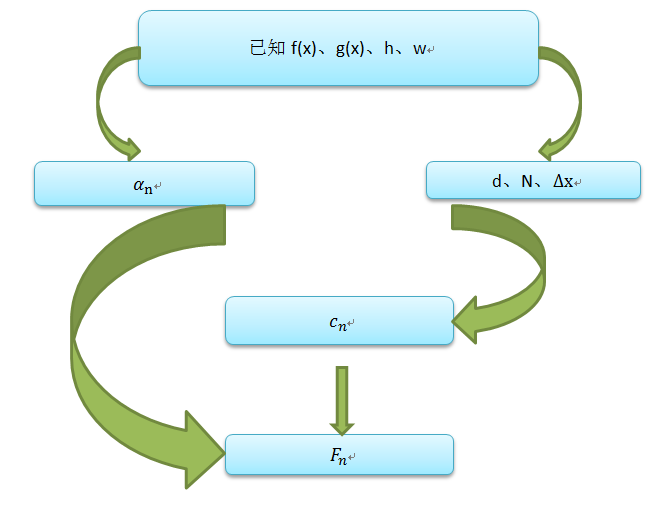
\includegraphics[width=.6\textwidth]{1.png}
	\caption{问题三流程图}
\end{figure}

\section{绘制普通三线表格}
表格应具有三线表格式,因此常用 booktabs宏包,其标准格式如表~\ref{tab001}~所示。
\begin{table}[!htbp]
	\caption{标准三线表格}\label{tab001} \centering
	\begin{tabular}{ccccc}
		\toprule[1.5pt]
		$D$(in) & $P_u$(lbs) & $u_u$(in) & $\beta$ & $G_f$(psi.in)\\
		\midrule[1pt]
		5 & 269.8 & 0.000674 & 1.79 & 0.04089\\
		10 & 421.0 & 0.001035 & 3.59 & 0.04089\\
		20 & 640.2 & 0.001565 & 7.18 & 0.04089\\
		\bottomrule[1.5pt]
	\end{tabular}
\end{table}

%插入.pdf/.esp图片
\begin{figure*} 
	\centering 
	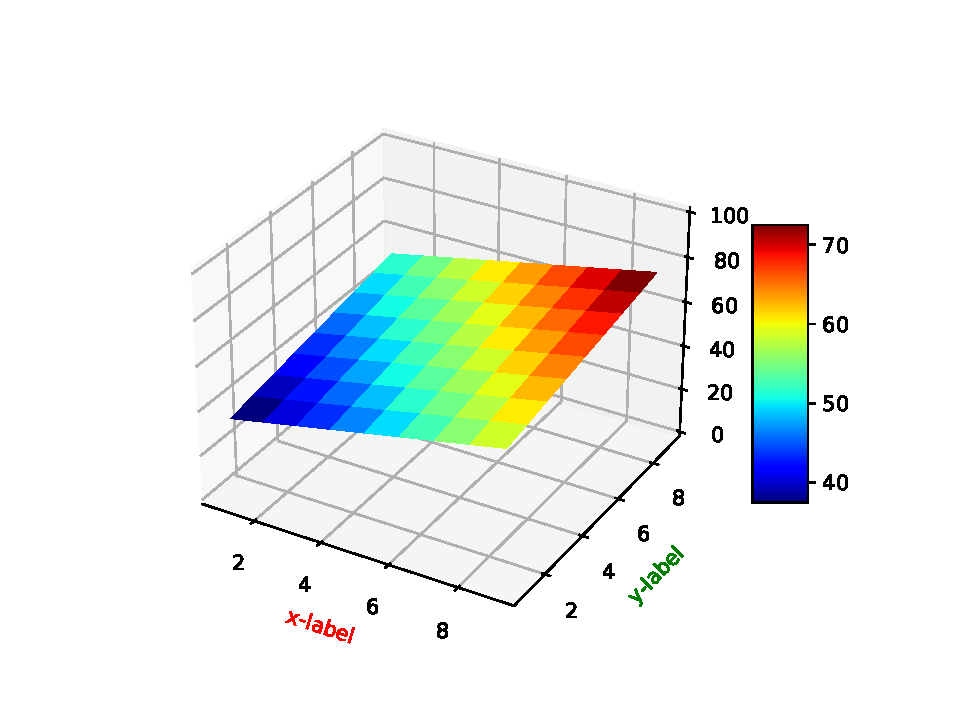
\includegraphics[width=.5\textwidth]{test_Figure.pdf}
	\caption{Results on…}
\end{figure*}

\begin{figure}
	\centering    
	\subfigure[子图一的标题]{				% 图片1([]内为子图标题)
		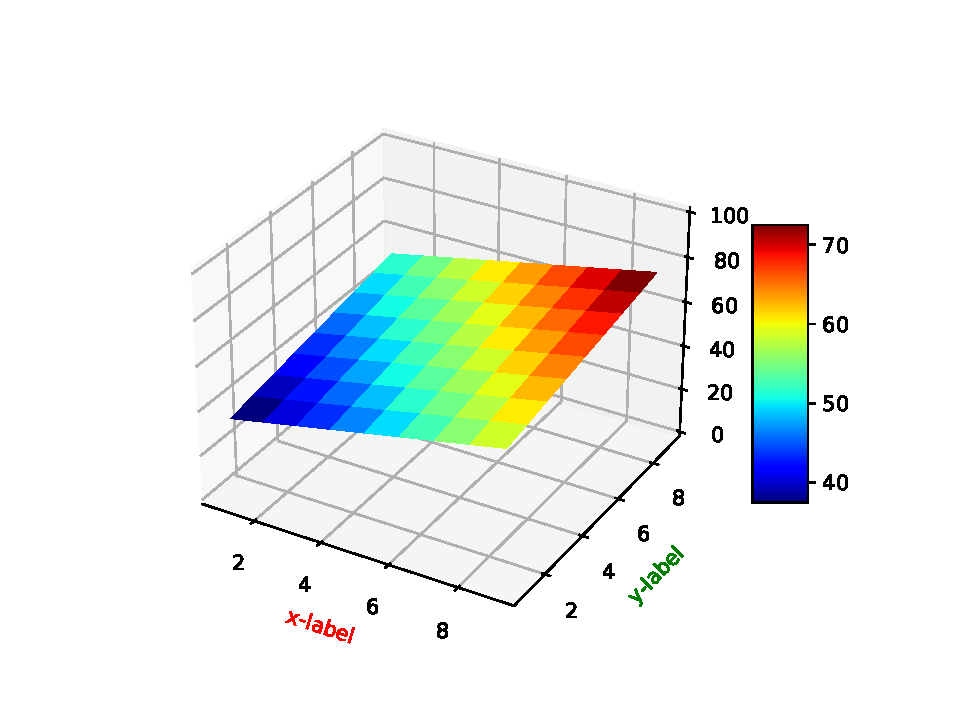
\includegraphics[width=0.45\textwidth]{test_Figure.pdf}}% 子图1的相对位置
	\subfigure[子图二的标题]{				% 图片2
		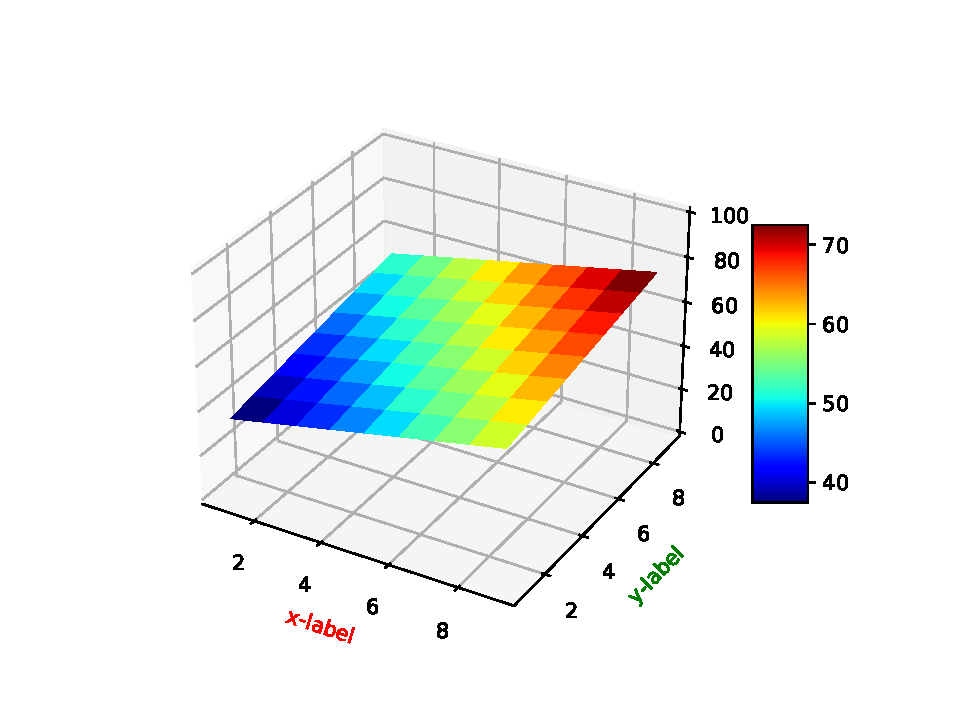
\includegraphics[width=0.45\textwidth]{test_Figure.pdf}}% 子图2的相对位置
	\caption{总图标题}		% 总图标题
\end{figure}

\begin{figure}
	\centering    
	\subfigure[子图一的标题]{				% 图片1([]内为子图标题)
		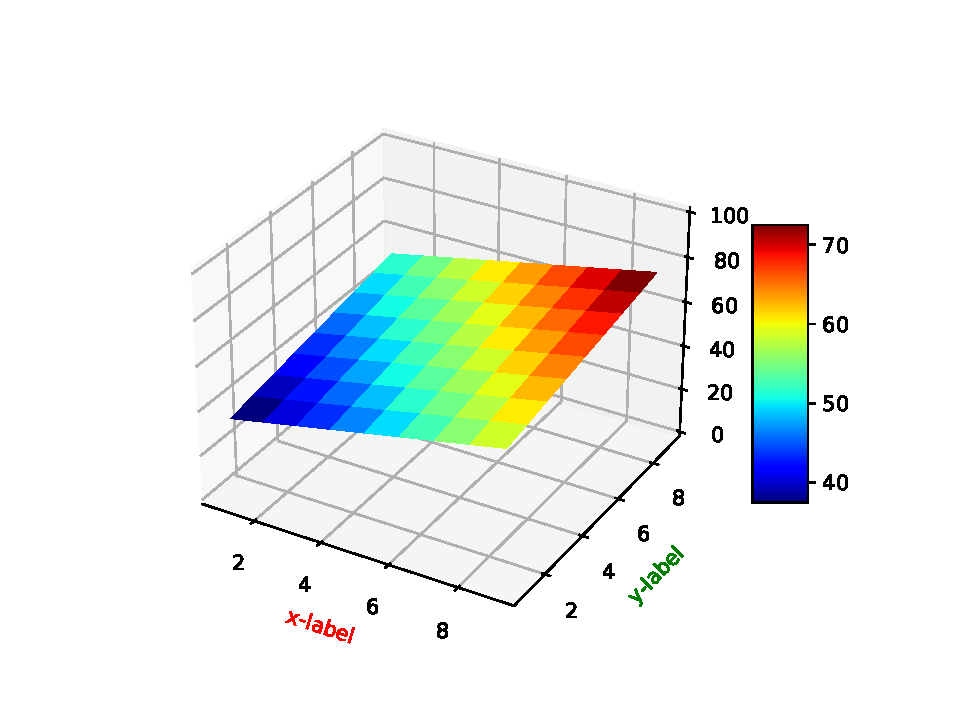
\includegraphics[width=0.3\textwidth]{test_Figure.pdf}}% 子图1的相对位置
	\subfigure[子图二的标题]{				% 图片2
		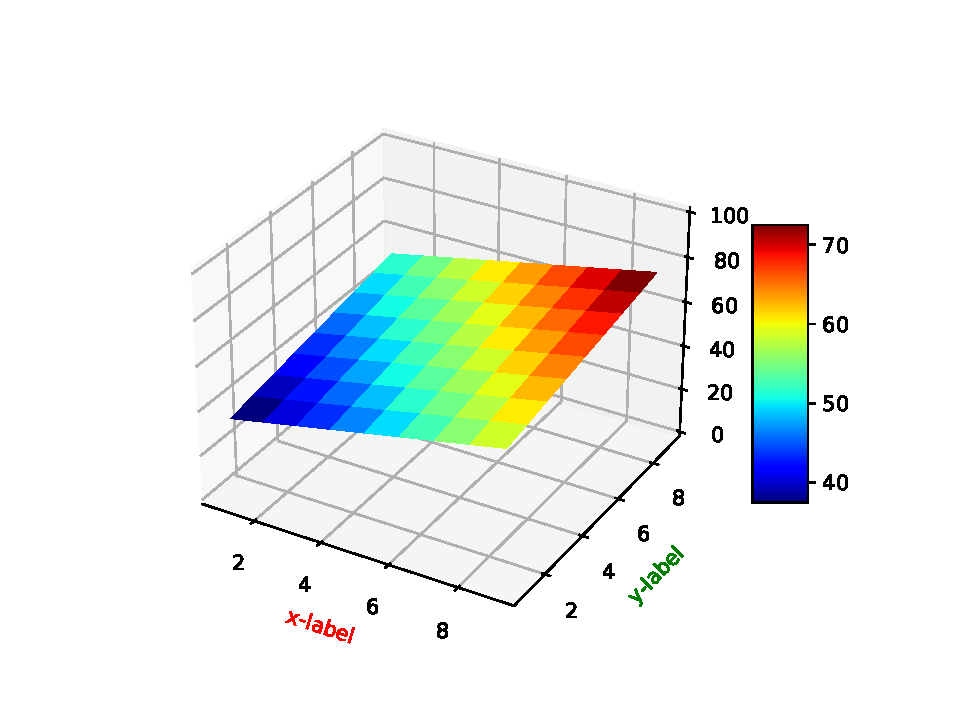
\includegraphics[width=0.3\textwidth]{test_Figure.pdf}}% 子图2的相对位置
	\subfigure[子图三的标题]{				% 图片2
		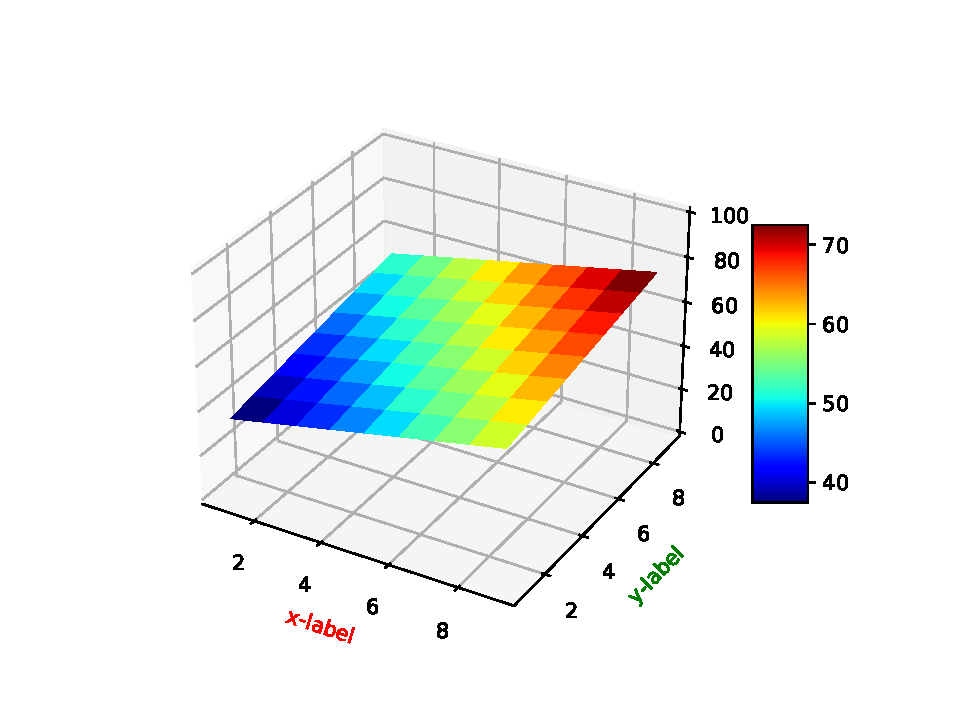
\includegraphics[width=0.3\textwidth]{test_Figure.pdf}}% 子图3的相对位置
	\caption{总图标题}		% 总图标题
\end{figure}



\newpage

\begin{center}
	$\max V, V \in(65,100) .$
	
	s.t. $\begin{cases}\text { 温度变化限制; } \quad & -3 \leq \frac{\partial u\left(\frac{d}{2}, t\right)}{\partial t} \leq 3 . 
		\\ \text { 温度区间限制: } & \left\{\begin{array}{l}u\left(\frac{d}{2}, t_{1}\right)=150, u\left(\frac{d}{2}, t_{2}\right)=190, \\ u\left(\frac{d}{2}, t_{3}\right)=217, u\left(\frac{d}{2}, t_{4}\right)=217, \\ 60 \leq t_{2}-t {1} \leq 120 . \\ 40 \leq t_{4}-t {3} \leq 90 .\end{array}\right. 
		\\ \text { 峰值温度限制; } \quad & 240 \leq \max u\left(\frac{d}{2}, t\right) \leq 250 .\end{cases}$
\end{center}

\begin{equation}
	\begin{gathered}
		\max V, V \in(65,100) . \\
		\text { s.t. } \begin{cases}\text { 温度变化限制; } \quad & -3 \leq \frac{\partial u\left(\frac{d}{2}, t\right)}{\partial t} \leq 3 . \\
			\text { 温度区间限制: } & \left\{\begin{array}{l}
				u\left(\frac{d}{2}, t_{1}\right)=150, u\left(\frac{d}{2}, t_{2}\right)=190, \\
				u\left(\frac{d}{2}, t_{3}\right)=217, u\left(\frac{d}{2}, t_{4}\right)=217, \\
				60 \leq t_{2}-t 1 \leq 120 . \\
				40 \leq t_{4}-t 3 \leq 90 .
			\end{array}\right. \\
			\text { 峰值温度限制; } \quad &240 \leq \max u\left(\frac{d}{2}, t\right) \leq 250 .\end{cases}
	\end{gathered}
\end{equation}

%mathtype编辑的公式要删掉前面的
\begin{equation}
	\left\{ \begin{array}{l}
		h;\\
		h;\\
		j;\\
		u;
	\end{array} \right.
\end{equation}

%伪代码
\begin{algorithm} 
	\caption{Calculate $y = x^n$} 
	\label{alg3} 
	\begin{algorithmic}
		\REQUIRE $n \geq 0 \vee x \neq 0$ 
		\ENSURE $y = x^n$ 
		\STATE $y \gets 1$ 
		\IF{$n < 0$} 
		\STATE $X \gets 1 / x$ 
		\STATE $N \gets -n$ 
		\ELSE 
		\STATE $X \gets x$ 
		\STATE $N \gets n$ 
		\ENDIF 
		\WHILE{$N \neq 0$} 
		\IF{$N$ is even} 
		\STATE $X \gets X \times X$ 
		\STATE $N \gets N / 2$ 
		\ELSE[$N$ is odd] \STATE $y \gets y \times X$ 
		\STATE $N \gets N - 1$ 
		\ENDIF 
		\ENDWHILE 
	\end{algorithmic} 
\end{algorithm}

\begin{algorithm}
	%\textsl{}\setstretch{1.8}
	\renewcommand{\algorithmicrequire}{\textbf{Input:}}
	\renewcommand{\algorithmicensure}{\textbf{Output:}}
	\caption{STVMD based on STFT}
	\label{alg1}
	\begin{algorithmic}[1]
		\STATE Initialization:$\left\{ {s_{k,t}^1} \right\},\left\{ {\omega _{k,t}^1} \right\},\lambda _t^1,n \leftarrow 0$
		\STATE  ${s_{r,t}}\left( \omega  \right) = \int_0^{ + \infty } {{s_r}\left( \tau  \right){w_h}\left( {t - \tau } \right)} \exp \left( {j\omega \tau } \right)d\tau $   (via STFT)
		\REPEAT
		\STATE $n \leftarrow n + 1$
		\STATE Update $ s_{k,t}^{n + 1} $ based on Equation~(\ref{eqn_8})
		\STATE Update $\omega _{k,t}^{n + 1}$ based on Equation~(\ref{eqn_9})
		\STATE Update $\lambda _t^{n + 1} $ based on Equation~(\ref{eqn_10})
		\UNTIL $\sum\limits_{k=1}^P  {{{\left\| {s_{k,t}^{n + 1}\left( \omega  \right) - s_{k,t}^n\left( \omega  \right)} \right\|_2^2} \mathord{\left/
					{\vphantom {{\left\| {s_{k,t}^{n + 1}\left( \omega  \right) - s_{k,t}^n\left( \omega  \right)} \right\|_2^2} {\left\| {s_{k,t}^n\left( \omega  \right)} \right\|_2^2}}} \right.
					\kern-\nulldelimiterspace} {\left\| {s_{k,t}^n\left( \omega  \right)} \right\|_2^2}}}  < \varepsilon $  
		\STATE   Update ${s_k}\left( t \right)$ based on Equation~(\ref{eqn_11_12})  (via ISTFT)
		\ENSURE  decomposed modes $ \left\{ {{s_k}\left( t \right)} \right\}$, $\left\{ {{\omega _k}\left( t \right)} \right\}$
	\end{algorithmic}  
\end{algorithm}
%%



\newpage
%参考文献
\begin{thebibliography}{9}%宽度9
	\bibitem{bib:one} GAO L, GONDA I, SUN H, et al. The Tomato Pan-Genome Uncovers New Genes and a	Rare Allele Regulating Fruit Flavor[J]. Nature Genetics, 2019:1.
	\bibitem{bib:two} 姚树坤, 倪晓昌, 杨旭, 等. 基于电子元器件称重的高精度电子称设计与实现[J]. 智能计算机与应用, 2017, 7(5): 142-145.
	\bibitem{bib:three} 姚树坤, 倪晓昌, 杨旭, 等. 基于电子元器件称重的高精度电子称设计与实现[J]. 智能计算机与应用, 2017, 7(5): 142-145.
\end{thebibliography}
\newpage
\appendix %%附录

\section{代码}
\subsection{排队算法--matlab 源程序}
\begin{lstlisting}[language=matlab]
kk=2;[mdd,ndd]=size(dd);
while ~isempty(V)
[tmpd,j]=min(W(i,V));tmpj=V(j);
for k=2:ndd
[tmp1,jj]=min(dd(1,k)+W(dd(2,k),V));
tmp2=V(jj);tt(k-1,:)=[tmp1,tmp2,jj];
end
tmp=[tmpd,tmpj,j;tt];[tmp3,tmp4]=min(tmp(:,1));
if tmp3==tmpd, ss(1:2,kk)=[i;tmp(tmp4,2)];
else,tmp5=find(ss(:,tmp4)~=0);tmp6=length(tmp5);
if dd(2,tmp4)==ss(tmp6,tmp4)
ss(1:tmp6+1,kk)=[ss(tmp5,tmp4);tmp(tmp4,2)];
else, ss(1:3,kk)=[i;dd(2,tmp4);tmp(tmp4,2)];
end;end
dd=[dd,[tmp3;tmp(tmp4,2)]];V(tmp(tmp4,3))=[];
[mdd,ndd]=size(dd);kk=kk+1;
end; S=ss; D=dd(1,:);
\end{lstlisting}
\subsection{规划解决程序--lingo源代码}
\begin{lstlisting}[language=c]
kk=2;
[mdd,ndd]=size(dd);
while ~isempty(V)
[tmpd,j]=min(W(i,V));tmpj=V(j);
for k=2:ndd
[tmp1,jj]=min(dd(1,k)+W(dd(2,k),V));
tmp2=V(jj);tt(k-1,:)=[tmp1,tmp2,jj];
end
tmp=[tmpd,tmpj,j;tt];[tmp3,tmp4]=min(tmp(:,1));
if tmp3==tmpd, ss(1:2,kk)=[i;tmp(tmp4,2)];
else,tmp5=find(ss(:,tmp4)~=0);tmp6=length(tmp5);
if dd(2,tmp4)==ss(tmp6,tmp4)
ss(1:tmp6+1,kk)=[ss(tmp5,tmp4);tmp(tmp4,2)];
else, ss(1:3,kk)=[i;dd(2,tmp4);tmp(tmp4,2)];
end;
end
dd=[dd,[tmp3;tmp(tmp4,2)]];V(tmp(tmp4,3))=[];
[mdd,ndd]=size(dd);
kk=kk+1;
end;
S=ss;
D=dd(1,:);
\end{lstlisting}


%插入python代码??
\lstset{language=python}

\lstset{
	%numbers=left, 
	%numberstyle= \tiny, 
	keywordstyle= \color{ blue!70},
	commentstyle= \color{red!50!green!50!blue!50}, 
	%frame=shadowbox, % 阴影效果
	rulesepcolor= \color{ red!20!green!20!blue!20} ,
	escapeinside=``, % 英文分号中可写入中文
	breaklines=true,   
	xleftmargin=2em, aboveskip=1em,
	framexleftmargin=2em
}
\noindent 对sonar数据集分类的代码如下: 
\begin{lstlisting}
	sum = 0
	for i in range(2,101,2):
	    sum += i
	print(sum)

\end{lstlisting}
\end{document}